\documentclass[12pt, letterpaper]{article}
\usepackage[top = 1cm, bottom = 0.75cm, left = 1in, right = 1in]{geometry}
\usepackage[utf8]{inputenc}
\usepackage[vietnamese]{babel}
\usepackage{graphicx}
\usepackage{amsmath}
\usepackage{titlesec}
\usepackage{color}
\usepackage{xcolor}
\usepackage{listings}
\usepackage{array}
\usepackage{adjustbox}
\geometry{margin=3cm}

\titleformat{\section}
{\Large\bfseries}
{Bài \thesection: }
{0em}
{}

\titleformat{\subsection}
{\large\bfseries}
{{\thesubsection} }
{0em}
{}

\renewcommand{\theenumi}{\bfseries\large\alph{enumi}}

\lstset{
  basicstyle=\ttfamily,
  mathescape
}

\title{
  \large\textbf{TRƯỜNG ĐẠI HỌC CÔNG NGHỆ THÔNG TIN} \\
  \large\textbf{KHOA KHOA HỌC MÁY TÍNH} \\
  \vfill
  \begin{figure}[h]
    \centering 
    
\includegraphics[width=0.5\linewidth]{uit} 
  \end{figure}
  \vfill
  \textbf{BÀI TẬP TUẦN 1} \\
  \textbf{MÔN\@: PHÂN TÍCH VÀ THIẾT KẾ THUẬT TOÁN}\\
  \vspace{1cm}
  \large \textcolor{blue}{\textbf{ĐÁNH GIÁ THUẬT TOÁN DÙNG KỸ THUẬT TOÁN SƠ CẤP \\}}
  \vfill
}

\author{
  \begin{tabular}{rl}
    \textbf{GV hướng dẫn:} &Huỳnh Thị Thanh Thương \\
    \textbf{Nhóm thực hiện:}
    &1. Võ Đình Khánh 22520659 \\
    &2. Nguyễn Gia Bảo 22520108 \\
    &3. Nguyễn Trần Phúc 22521135 \\
    &4. Hồ Trọng Duy Quang 22521200 \\
  \end{tabular}
}

\date{{\vfill}Thành phố Hồ Chí Minh, \MakeLowercase{\today}}

\begin{document}
\maketitle
\pagebreak
\newgeometry{margin=3cm}

\section{Tính tổng hữu hạn}

\subsection{Yêu cầu: Tính chính xác, không cho phép sai số hay xấp xỉ}
\begin{enumerate}
	\item $ \begin{aligned}[t]
			      1 + 3 + 5 + 7 + \cdots + 999
			       & = \sum^{499}_{i = 0} (2i + 1)                   \\
			       & = 2 \sum^{499}_{i = 0} i + \sum^{499}_{i = 0} 1 \\
			       & = 2 \frac{499(499 + 1)}{2} + (499 - 0 + 1)      \\
			       & = 250000                                        \\
		      \end{aligned} $

	\item $ \begin{aligned}[t]
			      2 + 4 + 8 + 16 + \cdots + 1024
			       & = \sum^{10}_{i = 1} 2^i       \\
			       & = \sum^{10}_{i = 0} 2^i - 2^0 \\
			       & = 2^{10 + 1} - 1 - 1          \\
			       & = 2046                        \\
		      \end{aligned} $

	\item $ \begin{aligned}
			      \sum^{n + 1}_{i = 3} 1 = (n + 1) - 3 + 1 = n - 1
		      \end{aligned} $

	\item $ \begin{aligned}[t]
			      \sum^{n + 1}_{i = 3} i & = \sum^{n + 1}_{i = 1} i - \sum^{2}_{i = 1} i   \\
			                             & = \frac{(n + 1)(n + 2)}{2} - \frac{2(2 + 1)}{2} \\
			                             & = \frac{n^2 + 3n - 4}{2}                        \\
		      \end{aligned} $

	\item $ \begin{aligned}[t]
			      \sum^{n - 1}_{i = 0} i(i + 1)
			       & = \sum^{n-1}_{i = 0} i^2 + \sum^{n - 1}_{i = 0} i \\
			       & = \sum^{n-1}_{i = 1} i^2 + \sum^{n - 1}_{i = 1} i \\
			       & = \frac{(n - 1)n(2n - 1)}{6} + \frac{(n - 1)n}{2} \\
			       & = \frac{n(n - 1)(n + 1)}{3}                       \\
		      \end{aligned} $

	\item $ \begin{aligned}[t]
			      \sum^{n}_{j = 1} 3^{j + 1}
			       & = 3\sum^{n}_{j = 1} 3^j            \\
			       & = 3[(\sum^{n}_{j = 0} 3^j) - 3^0]  \\
			       & = 3(\sum^{n}_{j = 0} 3^j) - 3      \\
			       & = 3\frac{3^{n + 1} - 1}{3 - 1} - 3 \\
			       & = \frac{3^{n + 2} - 9}{2}          \\
		      \end{aligned} $

	\item $ \begin{aligned}[t]
			      \sum^{n}_{i = 1} \sum^{n}_{j = 1} ij
			       & = \sum^{n}_{i = 1} i [\frac{n(n + 1)}{2}]     \\
			       & = \frac{n(n + 1)}{2} \cdot \frac{n(n + 1)}{2} \\
			       & = \frac{n^2{(n + 1)}^2}{4}
		      \end{aligned} $

	\item $ \begin{aligned}[t]
			      \sum^{n}_{i = 1} \frac{1}{i(i + 1)}
			       & = \sum^{n}_{i = 1} \frac{1}{i} - \sum^{n}_{i = 1} \frac{1}{i + 1}         \\
			       & = \sum^{n - 1}_{i = 0} \frac{1}{i + 1} - \sum^{n}_{i = 1} \frac{1}{i + 1} \\
			       & = 1 - \frac{1}{n + 1}
		      \end{aligned} $

	\item $ \begin{aligned}[t]
			      \sum_{j \in \{2, 3, 5\}} (j^2 + j) = (2^2 + 2) + (3^2 + 3) + (5^2 + 5) = 48
		      \end{aligned} $

	\item $ \begin{aligned}[t]
			      \sum^{m}_{i = 1} \sum^{n}_{j = 0} \sum^{100}_{k = 0} (i + j)
			       & = 101 \sum^{m}_{i = 1} \sum^{n}_{j = 0} (i + j)         \\
			       & = 101 \sum^{m}_{i = 1} [i(n + 1) + \frac{n(n + 1)}{2}]  \\
			       & = \frac{101m(n + 1)(m + 1)}{2} + \frac{101mn(n + 1)}{2} \\
			       & = \frac{101m(n + 1)(m + n + 1)}{2}
		      \end{aligned} $
\end{enumerate}

\subsection{Yêu cầu: Tính chính xác được thì tốt, không thì cho phép tính gần đúng/xấp xỉ}
\begin{enumerate}
	\item $ \begin{aligned}[t]
			      \sum^{n - 1}_{i = 0} {(i^2 + 1)}^2
			       & = \sum^{n - 1}_{i = 0} (i^4 + 2i^2 + 1)                                         \\
			       & = \sum^{n - 1}_{i = 0} i^4 + \sum^{n - 1}_{i = 0} 2i^2 + \sum^{n - 1}_{i = 0} 1 \\
			       & \approx \frac{n^{5}}{5} + \frac{(n - 1)n(2n - 1)}{6} + n                        \\
		      \end{aligned} $

	\item $ \begin{aligned}[t]
			      \sum^{n - 1}_{i = 2} \lg{i^2}
			       & = 2 \sum^{n - 1}_{i = 2} \lg{i}                 \\
			       & = 2 (\sum^{n - 1}_{i = 1} \lg{i} - \lg{1})      \\
			       & \approx 2 [(n - 1)\lg{(n - 1)} - (n - 1)\lg{1}] \\
			       & \approx 2 (n - 1)[\lg{(n - 1)} - \lg{1}]        \\
		      \end{aligned} $

	\item $ \begin{aligned}[t]
			      \sum^{n}_{i = 1} (i + 1)2^{i - 1}
			       & = \frac{\sum^{n}_{i = 1} (i2^i + 2^i)}{2}                  \\
			       & = \frac{[(n - 1)2^{n + 1} + 2] + [2^{n + 1} - 1 - 2^0]}{2} \\
			       & = (n - 1)2^n + 2^n                                         \\
			       & = n2^n
		      \end{aligned} $

	\item $ \begin{aligned}[t]
			      \sum^{n - 1}_{i = 0} \sum^{i - 1}_{j = 0} (i + j)
			       & = \sum^{n - 1}_{i = 0} (i^2 + \frac{(n - 1)n}{2})   \\
			       & = \frac{(n - 1)n(2n - 1)}{6} + \frac{n^2(n - 1)}{2} \\
		      \end{aligned} $
\end{enumerate}

\section{Đếm số phép gán và so sánh}

\begin{lstlisting}
    s = 0;                  $ 1g $
    i = 1;                  $ 1g $
    while ($ i \leq n $) do             $ (n + 1)ss $
        j = 1;              $ ng $
        while ($ j \leq i^2 $) do         $ (\alpha_i + 1)ss $
            s = s + 1;      $ \alpha_i g $
            j = j + 1;      $ \alpha_i g $
        end do;
        i = i + 1;          $ ng $
    end do;
  \end{lstlisting}

$ \begin{aligned}
		\text{Gọi } & \alpha_i \text{ là số lần lặp của while trong:}                              \\
		            & \alpha_i = \text{số con j chạy từ 1} \rightarrow i^2 \text{, bước tăng là 1} \\
		            & \alpha_i = i^2 - 1 + 1                                                       \\
		            & \alpha_i = i^2
	\end{aligned} $

\begin{align*}
	\text{Gán}(n) & = 2 + 2n + \sum^{n}_{i = 1} 2 \alpha_i \\
	              & = 2 + 2n + 2 \sum^{n}_{i = 1} i^2      \\
	              & = 2 + 2n + \frac{n(n + 1)(2n + 1)}{3}
\end{align*}

\begin{align*}
	SS(n) & = n + 1 + \sum^{n}_{i = 1} (\alpha_i + 1)           \\
	      & = n + 1 + \sum^{n}_{i = 1} i^2 + \sum^{n}_{i = 1} 1 \\
	      & = n + 1 + \frac{n(n + 1)(2n + 1)}{6} + n            \\
	      & = 2n + 1 + \frac{n(n + 1)(2n + 1)}{6}
\end{align*}

\section{Đếm số phép gán và so sánh}

\begin{lstlisting}
    float Alpha(float x, long n)
    {     long i = 1; float z = 0;          $ 2g $
          while ($ i \leq n $)                          $ (n + 1)ss $
          {       long j = 1; float t = 1;  $ 2ng $
                  while ($ j \leq i $)                  $ (\alpha_i + 1)ss $
                  {       t = t*x;          $ \alpha_i g $
                          j = 2*j;          $ \alpha_i g $
                  }
                  z = z+i*t;                $ ng $
                  i=i+1;                    $ ng $
          }
          return z;                         $ 1g $
    }
\end{lstlisting}

$ \begin{aligned}
		\text{Gọi } & \alpha_i \text{ là số lần lặp của while trong:}                              \\
		            & \alpha_i = \text{số con j chạy từ 1} \rightarrow i \text{, bước tăng theo tỉ lệ 2} \\
                    & j \in \{ 1, 2, 4, \ldots, 2^k \} \\
		            & \alpha_i = \text{đếm số con k:} \\
	\end{aligned} $ \\

\begin{align*}
    & 1 \leq 2^k \leq i \\
    \Leftrightarrow\; & 0 \leq k \leq \log_2{i} \\
    \Rightarrow\; & k = \log_2{i} + 1
\end{align*}

\begin{align*}
    \text{Gán}(n) & = 3 + 4n + \sum^{n}_{i = 1} 2 \alpha_i \\
                  & = 3 + 4n + 2 \sum^{n}_{i = 1} (\log_2{i} + 1) \\
                  & = 3 + 6n + 2 \sum^{n}_{i = 1} \log_2{i} \\
                  & \approx 3 + 6n + 2 n \log_2{n} \\
\end{align*}

\begin{align*}
	SS(n) & = n + 1 + \sum^{n}_{i = 1} (\alpha_i + 1)           \\
          & = n + 1 + \sum^{n}_{i = 1} (\log_2{i} + 2)           \\
          & = 3n + 1 + \sum^{n}_{i = 1} \log_2{i}           \\
          & \approx 3n + 1 + n \log_2{n}           \\
\end{align*}


%%%%%%%%%%%%%%%%%%%%%%%%%%%%%%%%%%%%%%%%%%%%%%%%%%%%%%%%%%%%%%%%%%%%%%%%%%%%%%%%%%%
\section{Đếm số phép gán và so sánh:}
\section{Đếm số phép gán và so sánh:}
\section{Đếm số phép gán và so sánh:}
\section{Đếm số phép gán và so sánh:}
\section{Đếm số phép gán và so sánh:}
\section{Đếm số phép gán và so sánh:}
%%%%%%%%%%%%%%%%%%%%%%%%%%%%%%%%%%%%%%%%%%%%%%%%%%%%%%%%%%%%%%%%%%%%%%%%%%%%%%%%%%%
\section{Đếm số phép gán và so sánh:}

\begin{figure}[h]
	\centering
	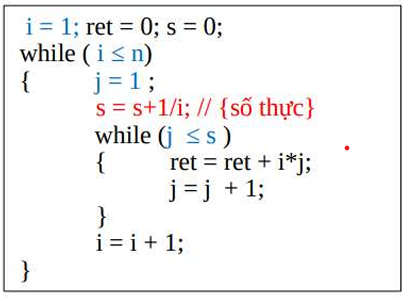
\includegraphics{Bai10}
\end{figure}
{\color{red} \emph{\textbf{Giải:}}}

\begin{flalign*}
	\text{Gọi } \alpha_i & \text{ là số vòng lặp của while trong}                        &  & \\
	                     & = \text{số con j chạy từ 1 } \rightarrow s = s + \dfrac{1}{i}
\end{flalign*}
Suy ra: $\alpha_i$ = s + $\dfrac{1}{i}$ - 1 + 1 = s + $\dfrac{1}{i}$ \\
Ta có: s $\in$ \{1 ; 1 + $\dfrac{1}{2}$ ; 1 + $\dfrac{1}{2}$ + $\dfrac{1}{3}$ ; … ; 1 + $\dfrac{1}{2}$ + $\dfrac{1}{3}$ + … + $\dfrac{1}{n}$ \} \\
Suy ra: $\alpha_i$ = $\sum_{k=1}^i \dfrac{1}{k}$, với i lần lượt là 1, 2, 3,..., n \\
\begin{flalign*}
	\text{Gán}(n) & = 3 + 3n + \sum_{i=1}^n 2\alpha_i                  &  & \\
	              & = 3 + 3n + 2\sum_{i=1}^n \sum_{k=1}^i \dfrac{1}{k} &  & \\
	\text{SS(n) } & = n + 1 + \sum_{i=1}^n (\alpha_i + 1)              &  & \\
	              & = 2n + 1 + \sum_{i=1}^n \sum_{k=1}^i \dfrac{1}{k}  &  & \\
\end{flalign*}

\pagebreak
\section{Cho n,m là các số nguyên dương. Xem xét thuật toán sau đây, giả sử phép gán và phép so sánh đóng vai trò chủ yếu trong thời gian chạy của thuật toán:}

\begin{figure}[h]
	\centering
	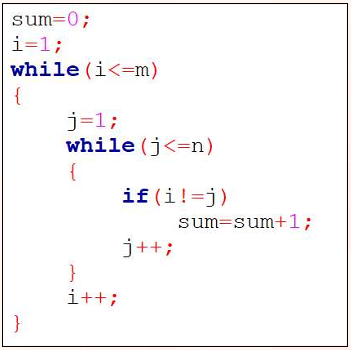
\includegraphics{Bai11}
\end{figure}
{\color{red} \emph{\textbf{Giải}}} \\
$\textbf{a)}$
\begin{flalign*}
	\text{Gọi } \alpha_i & \text{ là số lần lặp của while trong}            \\
	                     & \text{= số con j chạy từ 1 $\rightarrow$ n}      \\
	                     & \text{= n}                                  &  & \\
\end{flalign*}
Câu lệnh if(i!=j) được thực hiện mn lần, điều kiện của if chỉ sai khi i = j.
\begin{itemize}
	\item Trường hợp 1: $n \leq m$ \\
	      Trong mỗi vòng lặp của i trong khoảng [1, n], j cũng chạy trong khoảng [1, n], mỗi lần như vậy i = j một lần, tổng là n lần.
	      Suy ra: lệnh sum = sum + 1 được thực hiện (mn – n) lần
	\item Trường hợp 2: $n > m$ \\
	      Trong mỗi vòng lặp của i trong khoảng [1, m], j cũng chạy trong khoảng [1, m], mỗi lần như vậy i = j một lần, tổng là m lần.
	      Suy ra: lệnh sum = sum + 1 được thực hiện (mn – m) lần
\end{itemize}
Vậy: lệnh sum = sum + 1 được thực hiện (mn – min(m,n)) lần \\
\setlength{\baselineskip}{1.2\baselineskip}
Gán(n) = 2 + 2m + mn + (mn – min(m,n)) \\
So sánh(n) = m + 1 + m(n+1) + mn \\

\pagebreak
$\textbf{b)}$ \\
Chương trình C++:
\begin{lstlisting}[language=C++]
  	#include <iostream>
  	
  	int main() {
  		int m, n;
  		
  		std::cout << "Enter m: ";
  		std::cin >> m;
  		std::cout << "Enter n: ";
  		std::cin >> n;
  		
  		int s = 0;
  		int i = 1;
  		int demGan = 2;
  		int demSS = 0;
  		
  		while (i <= m) {
  			demSS += 1;
  			int j = 1;
  			while (j <= n) {
  				demSS += 1;
  				if (i != j) {
  					s = s + 1;
  					demGan += 1;
  				}
  				demSS += 1;
  				j += 1;
  				demGan += 1;
  			}
  			demSS += 1;
  			i += 1;
  			demGan += 2;
  		}
  		
  		demSS += 1;
  		
  		std::cout << "Gan(n) = " << demGan << std::endl;
  		std::cout << "SS(n) = " << demSS << std::endl;
  		
  		return 0;
  	}
  \end{lstlisting}

\pagebreak
\begin{figure}[!]
	\centering \large Kết quả chạy chương trình
	\caption{(10,20)}
	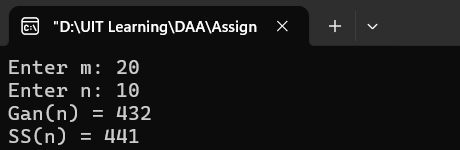
\includegraphics{Bai11_1}
	\caption{(35,24)}
	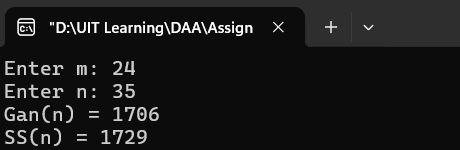
\includegraphics{Bai11_2}
	\caption{(50,50)}
	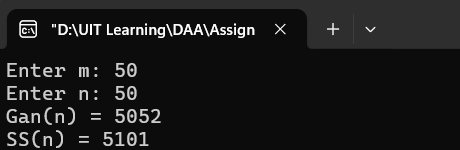
\includegraphics{Bai11_3}
	\caption{(200,100)}
	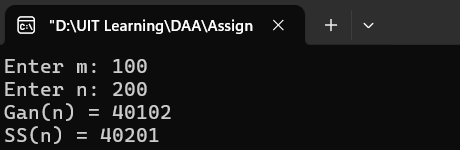
\includegraphics{Bai11_4}
	\caption{(100,200)}
	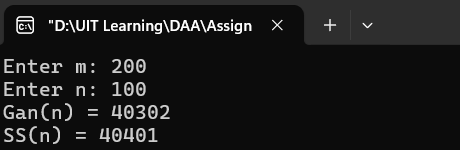
\includegraphics{Bai11_5}
\end{figure}

\pagebreak
\begin{center}
	\begin{tabular}{| m{10em} | m{1.5cm}| m{1.5cm} | m{1.5cm} | m{2cm} | m{2cm} |}
		\hline
		Ví dụ 5 bộ dữ liệu thử nghiệm (n, m)                  & (10, 20) & (35, 24) & (50, 50) & (200, 100) & (100, 200) \\
		\hline
		Gán(n) = …(theo công thức đếm thủ công từ câu a)      & 432      & 1706     & 5052     & 40102      & 40302      \\
		\hline
		Gán(n) kết quả khi chạy chương trình ở Bước 2         & 432      & 1706     & 5052     & 40102      & 40302      \\
		\hline
		So sánh(n) = …(theo  công thức đếm thủ công từ câu a) & 441      & 1729     & 5101     & 40201      & 40401      \\
		\hline
		So sánh(n) kết quả khi chạy chương trình              & 441      & 1729     & 5101     & 40201      & 40401      \\
		\hline
	\end{tabular}
\end{center}

\noindent Nhận xét kết quả so sánh: Số phép gán và số phép so sánh  khi tính bằng công thức từ câu a và khi chạy chương trình là bằng nhau.
\end{document}
